\documentclass{beamer}
\setbeamertemplate{footline}[page number]
\date{}
\author{}
\institute{}

%%%%%%% Put these names back in the final version 
%\\Aswathy Rajendra Kurup\\Meenu Ajith}
%\institute{Department of Electrical and Computer Engineering\\The University of New Mexico}
\setbeamercovered{transparent}
\usepackage{setspace}
\usepackage{array}
\usepackage[T1]{fontenc}
\usepackage{graphicx}
\usepackage{amsmath}
\usepackage{amsfonts}
\usepackage{amssymb}
\usepackage{makeidx}
\usefonttheme{serif}
\usepackage{multirow}
\usepackage{booktabs} 
\usepackage{rotating}
\usepackage{color}
\usepackage{float}
\usepackage[latin1]{inputenc}
\usepackage[english]{babel}
\usepackage{amsmath}
\usepackage{amsfonts}
\usepackage{eurosym}
\usepackage{rotating}
\usepackage{multicol}
\usepackage{pythonhighlight}
\usepackage[normalem]{ulem}
\newcommand{\ba}{{\bf a}}
\newcommand{\bb}{{\bf b}}
\newcommand{\bc}{{\bf c}}
\newcommand{\bd}{{\bf d}}
\newcommand{\be}{{\bf e}}
\newcommand{\bbf}{{\bf f}}
\newcommand{\bg}{{\bf g}}
\newcommand{\bh}{{\bf h}}
\newcommand{\bi}{{\bf i}}
\newcommand{\bk}{{\bf k}}
\newcommand{\bl}{{\bf l}}
\newcommand{\bm}{{\bf m}}
\newcommand{\bn}{{\bf n}}
\newcommand{\bo}{{\bf o}}
\newcommand{\bp}{{\bf p}}
\newcommand{\bq}{{\bf q}}
\newcommand{\br}{{\bf r}}
\newcommand{\bs}{{\bf s}}
\newcommand{\bt}{{\bf t}}
\newcommand{\bu}{{\bf u}}
\newcommand{\bv}{{\bf v}}
\newcommand{\bw}{{\bf w}}
\newcommand{\bx}{{\bf x}}
\newcommand{\by}{{\bf y}}
\newcommand{\bz}{{\bf z}}

\newcommand{\bA}{{\bf A}}
\newcommand{\bB}{{\bf B}}
\newcommand{\bC}{{\bf C}}
\newcommand{\bE}{{\bf E}}
\newcommand{\bG}{{\bf G}}
\newcommand{\bH}{{\bf H}}
\newcommand{\bI}{{\bf I}}
\newcommand{\bK}{{\bf K}}
\newcommand{\bL}{{\bf L}}
\newcommand{\bM}{{\bf M}}
\newcommand{\bO}{{\bf O}}
\newcommand{\bQ}{{\bf Q}}
\newcommand{\bR}{{\bf R}}
\newcommand{\bS}{{\bf S}}
\newcommand{\bT}{{\bf T}}
\newcommand{\bV}{{\bf V}}
\newcommand{\bW}{{\bf W}}
\newcommand{\bX}{{\bf X}}
\newcommand{\bY}{{\bf Y}}
\newcommand{\bZ}{{\bf Z}}
\newcommand\uptocnt{\stackrel{\mathclap{\normalfont\mbox{c}}}{\propto}}
\newcommand{\bpt}{{\bf pt}}
\newcommand{\bpl}{{\bf pl}}
\newcommand{\bdp}{{\bf dp}}
\newcommand{\btemp}{{\bf temp}}

\newcommand{\bmu}{{\boldsymbol \mu}}
\newcommand{\bSigma}{{\boldsymbol \Sigma}}
\newcommand{\bsigma}{{\boldsymbol \sigma}}
\newcommand{\bvarPhi}{{\boldsymbol \varPhi}}
\newcommand{\bvarphi}{{\boldsymbol \varphi}}
\newcommand{\bPhi}{{\boldsymbol \Phi}}
\newcommand{\bdelta}{{\boldsymbol \delta}}
\newcommand{\bZero}{{\bf 0}}
\newcommand{\bOne}{{\bf 1}}
\newcommand{\balpha}{{\boldsymbol \alpha}}
\newcommand{\bAlpha}{{\boldsymbol A}}
\newcommand{\btheta}{{\boldsymbol \theta}}

\newcommand{\softmax}{\text{softmax}}
\newcommand{\diag}{\text{diag}}
\newcommand{\sinc}{\mathrm{sinc}}
\newcommand{\argmin}{\mathop{\mathrm{argmin}}}
\newcommand{\infl}{\eta}
\newcommand{\Ind}{\mathrm{I}}
\newcommand{\Real}{\mathbb R}
\newcommand{\Intg}{\mathbb Z}
\newcommand{\Complex}{\mathbb C}
\newcommand{\Natural}{\mathbb N}
\newcommand{\Fourier}[1]{\mathcal{F} \{#1\}}
%\newcommand{\ii}{\mathbbm{i}}
\newcommand{\bphi}{\boldsymbol{\mathit{\phi}}}

\newcommand{\hs}{\hspace{2pt}}
\newcommand{\sign}{\text{sign}}
\author{Manel Mart\'inez-Ram\'on\\Meenu Ajith\\Aswathy Rajendra Kurup}

\usetheme{Madrid}
\usecolortheme{beaver}
\usepackage{tikz}
\usetikzlibrary{fit,arrows,calc,positioning}
\usepackage{listings}
\usepackage{xcolor}
\usepackage{emerald} 
\usepackage[T1]{fontenc} 
\usepackage{verbatim}
\usepackage{graphicx}
\usepackage{epsfig}
\usepackage{psfrag}
\usepackage[english]{babel}
\usepackage{listings}
\usepackage{courier}
\usepackage{color}
 \usepackage{vwcol} 
 \usepackage[english]{babel} % To obtain English text with the blindtext package
\usepackage{blindtext}
\definecolor{codegreen}{rgb}{0,0.6,0}
\definecolor{codegray}{rgb}{0.5,0.5,0.5}
\definecolor{codepurple}{rgb}{0.58,0,0.82}
\definecolor{backcolour}{rgb}{0.95,0.95,0.92}

\lstdefinestyle{mystyle}{
  backgroundcolor=\color{backcolour},   commentstyle=\color{codegreen},
  keywordstyle=\color{magenta},
  numberstyle=\tiny\color{codegray},
  stringstyle=\color{codepurple},
  basicstyle=\ttfamily\footnotesize,
  breakatwhitespace=false,         
  breaklines=true,                 
  captionpos=b,                    
  keepspaces=true,                 
  numbers=left,                    
  numbersep=5pt,                  
  showspaces=false,                
  showstringspaces=false,
  showtabs=false,                  
  tabsize=2
}
\lstset{style=mystyle}

%% Stuff for movies

% %\newcommand{\bt}{{\bf t}}
% \newcommand{\br}{{\bf r}}
% \newcommand{\bs}{{\bf s}}
% \newcommand{\by}{{\bf y}}
% \newcommand{\bz}{{\bf z}}
% \newcommand{\bx}{{\bf x}}
% \newcommand{\bw}{{\bf w}}
% \newcommand{\be}{{\bf e}}
% \newcommand{\bbf}{{\bf f}}
% \newcommand{\bb}{{\bf b}}
% \newcommand{\bd}{{\bf d}}
% \newcommand{\bA}{{\bf A}}
% \newcommand{\bB}{{\bf B}}
% \newcommand{\bL}{{\bf L}}
% \newcommand{\bM}{{\bf M}}

% \newcommand{\bC}{{\bf C}}
% \newcommand{\bI}{{\bf I}}
% \newcommand{\bK}{{\bf K}}
% \newcommand{\bk}{{\bf k}}
% \newcommand{\bT}{{\bf T}}
% \newcommand{\bV}{{\bf V}}
% \newcommand{\bW}{{\bf W}}
% \newcommand{\bX}{{\bf X}}
% \newcommand{\bY}{{\bf Y}}
% \newcommand{\bZ}{{\bf Z}}
% \newcommand{\bm}{{\bf m}}
% \newcommand{\bpt}{{\bf pt}}
% \newcommand{\bpl}{{\bf pl}}
% \newcommand{\bdp}{{\bf dp}}
% \newcommand{\btemp}{{\bf temp}}
% \newcommand{\bl}{{\bf l}}
% \newcommand{\bu}{{\bf u}}
% \newcommand{\bmu}{{\boldsymbol \mu}}
% \newcommand{\bSigma}{{\boldsymbol \Sigma}}
% \newcommand{\bLambda}{{\boldsymbol \Lambda}}

% \newcommand{\bsigma}{{\boldsymbol \sigma}}
% \newcommand{\bvarphi}{{\boldsymbol \varPhi}}
% \newcommand{\btheta}{{\boldsymbol \theta}}
% \newcommand{\bZero}{{\bf 0}}
% \newcommand{\balpha}{{\boldsymbol \alpha}}
% \newcommand{\bpi}{{\boldsymbol \pi}}
% \newcommand{\bxi}{{\boldsymbol \xi}}
% \newcommand{\bdelta}{{\boldsymbol \delta}}
\lstset{
	language=Python,
	basicstyle=\footnotesize\ttfamily\color{black},
	commentstyle = \footnotesize\ttfamily\color{red},
	keywordstyle=\footnotesize\ttfamily\color{blue},
	stringstyle=\footnotesize\ttfamily\color{black},
%	columns=fixed,
%	numbers=left,    
	numberstyle=\tiny,
	stepnumber=1,
	numbersep=5pt,
	tabsize=1,
	extendedchars=true,
	breaklines=true,            
	frame=b,         
	showspaces=false,
	showtabs=true,
	xleftmargin=6pt,
	framexleftmargin=6pt,
	framexrightmargin=2pt,
	framexbottommargin=4pt,
	showstringspaces=false      
}

\lstloadlanguages{
         Python
}

%\graphicspath{ {./images/} }  % Figures path - used in graphicx

%\selectcolormodel{cmyk}

\mode<presentation>

\newcommand{\dred}{darkred!90!black}
\newcommand{\written}{\ECFJD\textcolor{cyan!50!white}}
\newcommand{\hlight}{\textcolor{\dred}}
\newcommand{\Ex}{\textcolor{\dred}{Ex. }}

% remove navigation symbols in full screen mode
\setbeamertemplate{navigation symbols}{}  
\setbeamertemplate{blocks}[rounded][shadow=false]
\setbeamercolor{note page}{fg=black}

\setbeamercolor{title}{fg=\dred}
\setbeamercolor{frametitle}{fg=white}
\setbeamercolor{frametitle}{bg=\dred}
\setbeamercolor{structure}{fg=black,bg=white}
\setbeamercolor{background canvas}{bg=white,fg=black}
\setbeamercolor{normal text}{fg=black,bg=white}
\setbeamercolor{item}{fg=red!80!black,bg=white!}
\addtobeamertemplate{block begin}{\setbeamercolor{block title}{fg=white,bg=\dred}
\setbeamercolor{block body}{fg=white,bg=gray}}{}


\title{5. Sequence modeling with recurrent neural networks}
\subtitle{5.4. Long Short-Term Memory Networks}

\addtobeamertemplate{frametitle}{}

\begin{document}
\maketitle

\begin{frame}{Introduction}
\begin{itemize} 

\item Short-term dependencies can be stored by RNNs , but long-time ones cannot be captured due to the exploding and vanishing gradient phenomena in BPTT 
\item The LSTMs  is a variation of RNNs that can handle long-term connections. 
\item Introduced by Sepp Hochreiter and J\"urgen Schmidhuber in 1997 to tackle the problems posed by standard RNNs.
\item The LSTM passes a linear  internal state from one time instant to the next one with unit gain to propagate the gradient without exploding or vanishing. 
\item In the original LSTM paper by Hochreiter and Schmidhuber this mechanism is called constant error carousel (CEC).  
\end{itemize}
\end{frame}

\begin{frame}{Structure}{This really is an LSTM}
\begin{center}
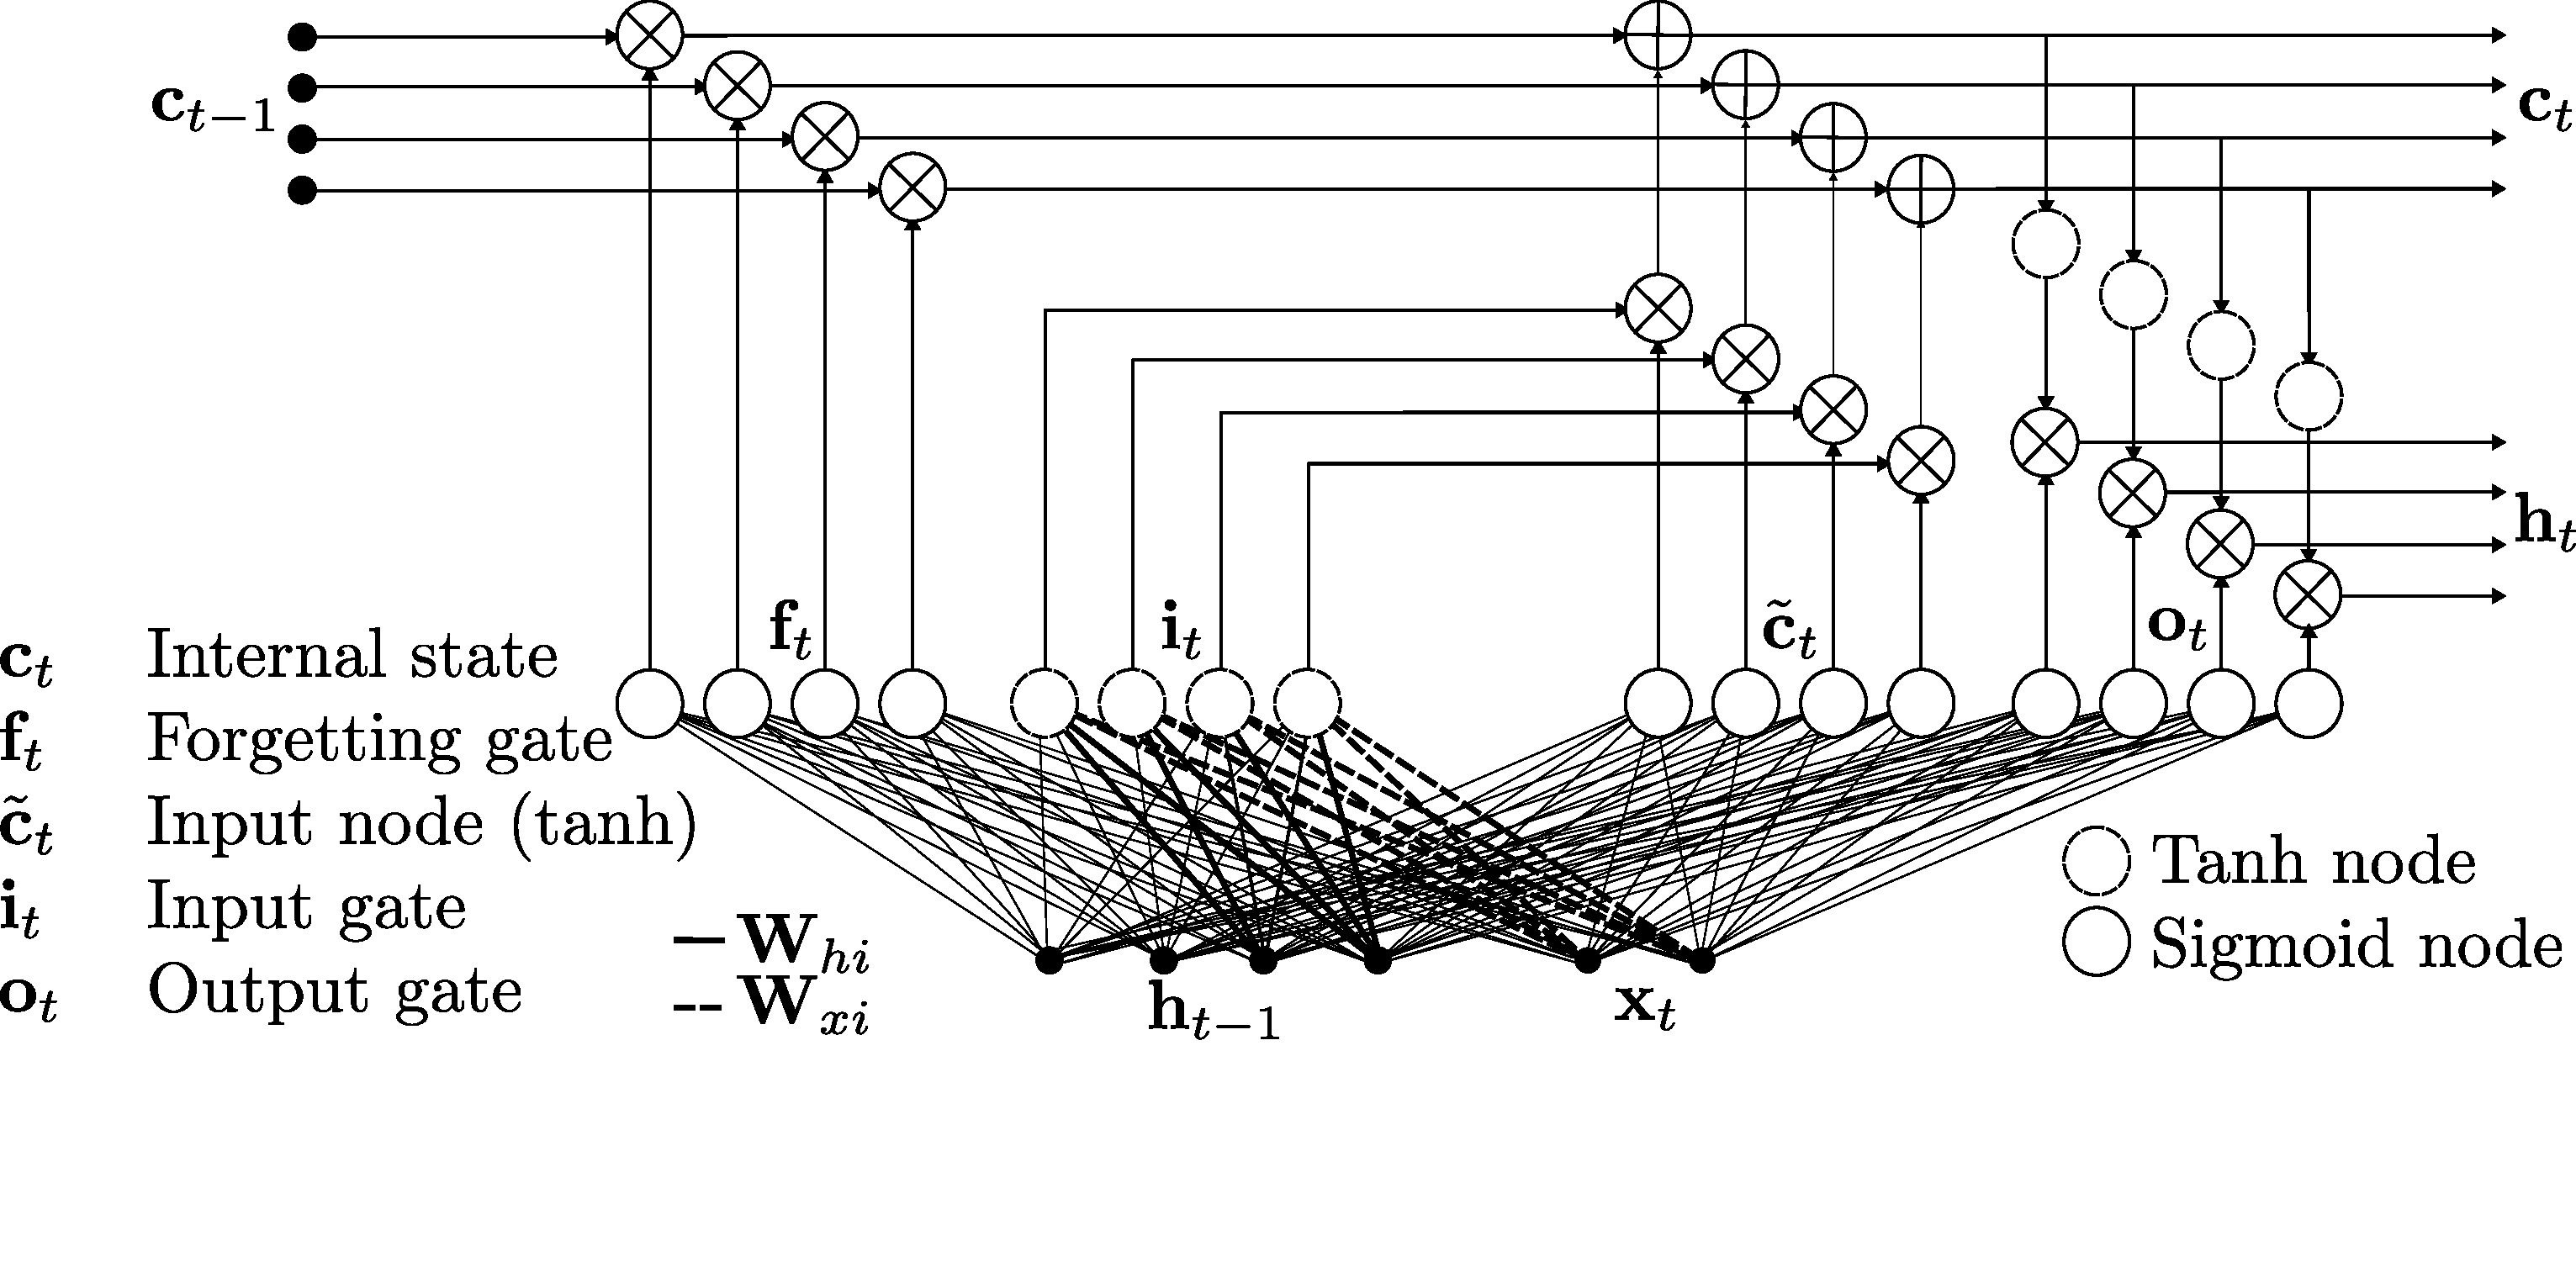
\includegraphics[scale=0.22]{Module 5 (RNN)/pics/LSTM_gates_as_NN.pdf}    
\end{center}
\end{frame}
\begin{frame}{Structure}{Compact (and more reasonable) structure representation}
\begin{center}
    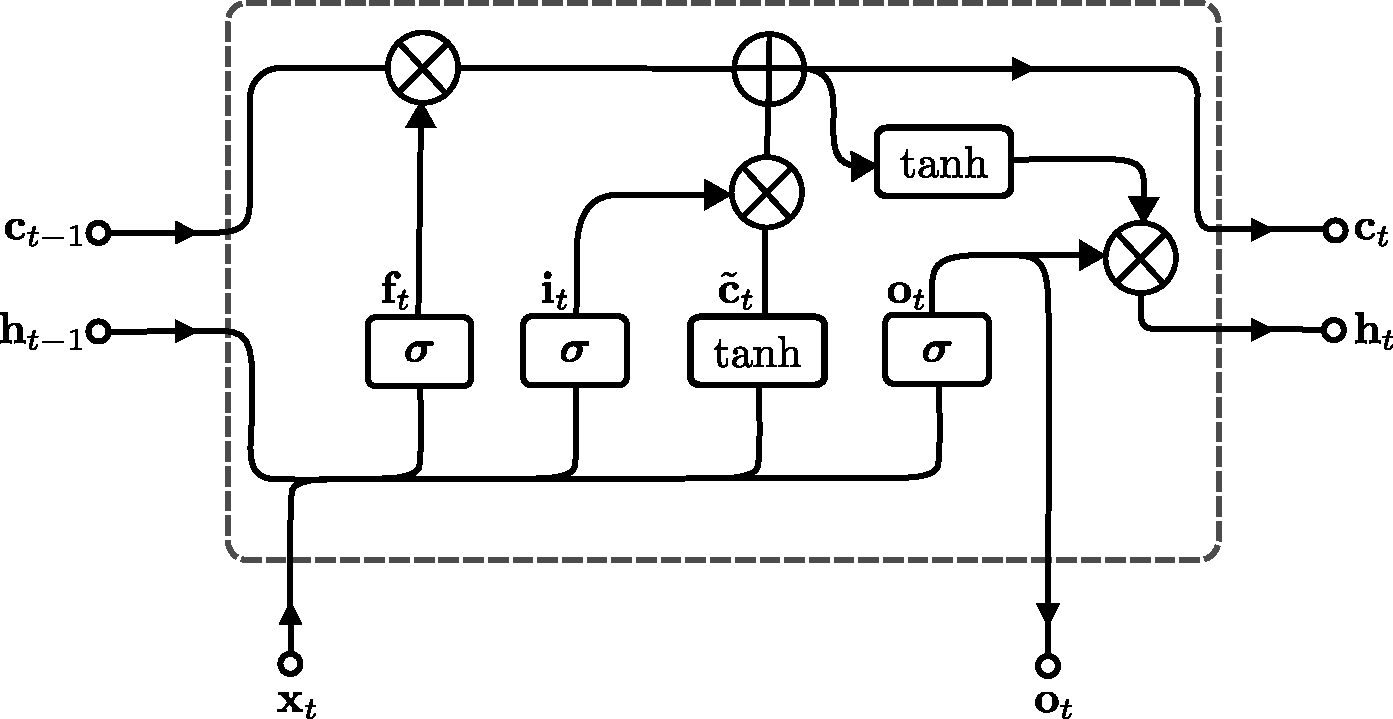
\includegraphics[scale=0.4]{ Module 5 (RNN)/pics/Long_Short-Term_Memory.pdf}
\end{center}
\end{frame}
\begin{frame}{Structure}{LSTM gates}
\begin{itemize}
\item The LSTM inputs are the internal state  $\bc_{t-1}$, the hidden state $\bh_{t-1}$, and the present input pattern $\bx_t$. 
\item The LSTM unit computes the values of the forgetting gate $\bbf_t$, the input gate $\bi_t$, and the output gate $\bo_t$. 
\item The expressions of these three activations are:
   \end{itemize} 
\begin{multicols}{2}

\begin{center}
    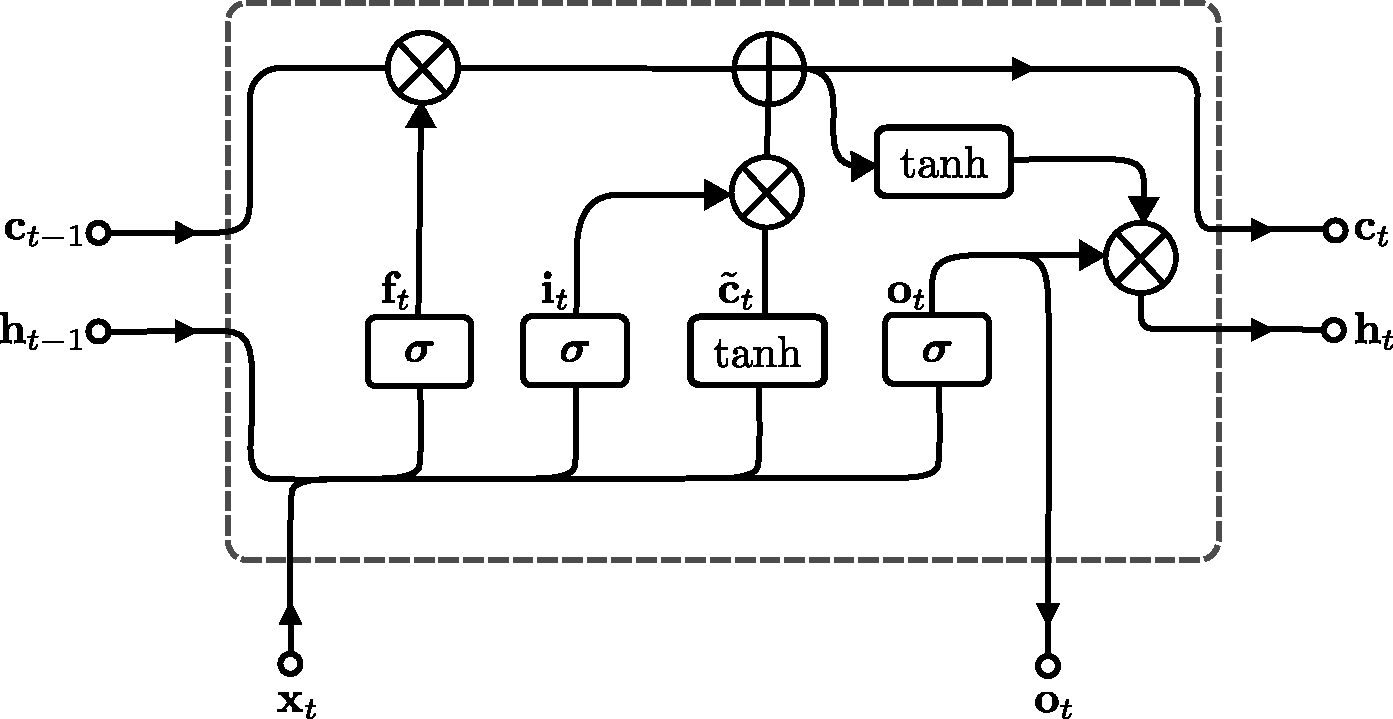
\includegraphics[scale=0.25]{ Module 5 (RNN)/pics/Long_Short-Term_Memory.pdf}
\end{center}

\columnbreak 

\begin{equation}
    \begin{split}
        \bbf_t & = \bsigma\left(\bW_{xf}^\top \bx_i +\bW_{hf}\bh_{t-1} + \bb_f\right)\\
        \bi_t & = \bsigma\left(\bW_{xi}^\top \bx_i +\bW_{hi}\bh_{t-1} + \bb_i\right)\\
        \bo_t & = \bsigma\left(\bW_{xo}^\top \bx_i +\bW_{ho}\bh_{t-1} + \bb_o\right)\\
    \end{split}
\end{equation}

\end{multicols}
 
\end{frame}

\begin{frame}{Structure}{LSTM gates $\bbf_t$, $\bi_t$, and $\bo_t$}
\begin{center}
 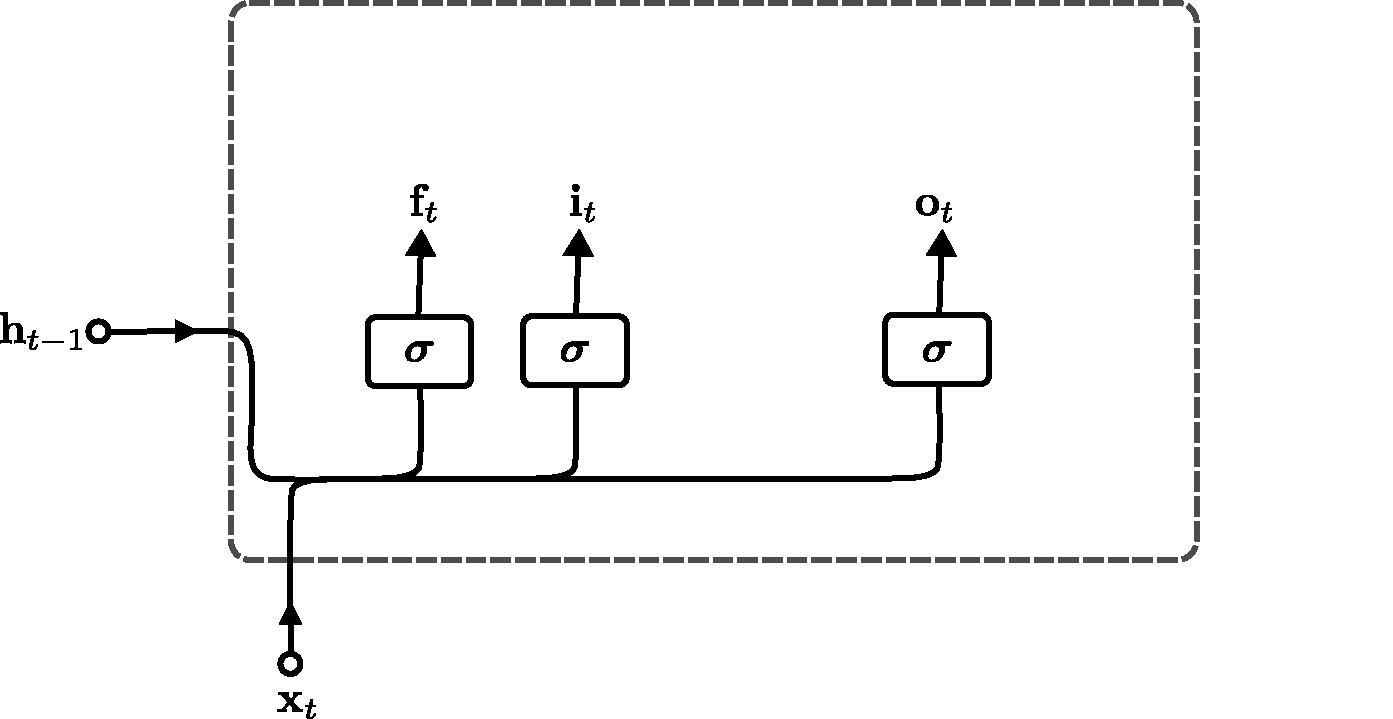
\includegraphics[scale=0.4]{Module 5 (RNN)/pics/LSTM_gates.pdf}
 \end{center}
 \begin{itemize}
     \item $\bbf_t$ is trained to forget the previous internal state if necessary. 
     \item $\bi_t$ determines how much of the input must be used to modify $\bc_t$. 
     \item $\bo_t$  will modulate $\bc_t$ to compute state $\bh_t$.
 \end{itemize}
\end{frame}

\begin{frame}{Structure}{Input gate  $\tilde{\bc}_t$}
\begin{center}
 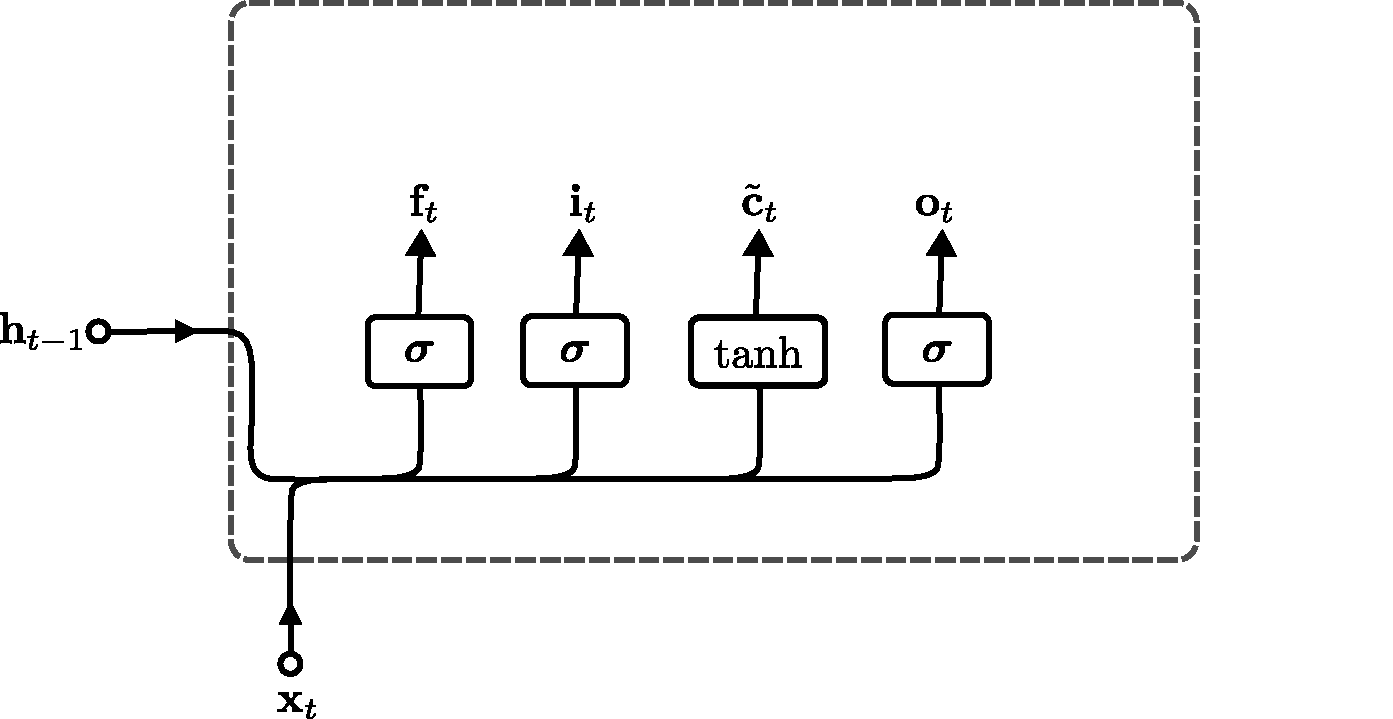
\includegraphics[scale=0.4]{Module 5 (RNN)/pics/LSTM_int_stat.pdf}
 \end{center}   
 \begin{equation}
    \tilde{\bc}_t = \bsigma\left(\bW_{xc}^\top \bx_i +\bW_{hc}\bh_{t-1} + \bb_c\right)
\end{equation}
 \begin{itemize}
\item $\tilde{\bc}_t$ is used to update the previous internal state. 
\end{itemize}
\end{frame}
\begin{frame}{Structure}{Internal state  $\bc_t$}
    \begin{center}
 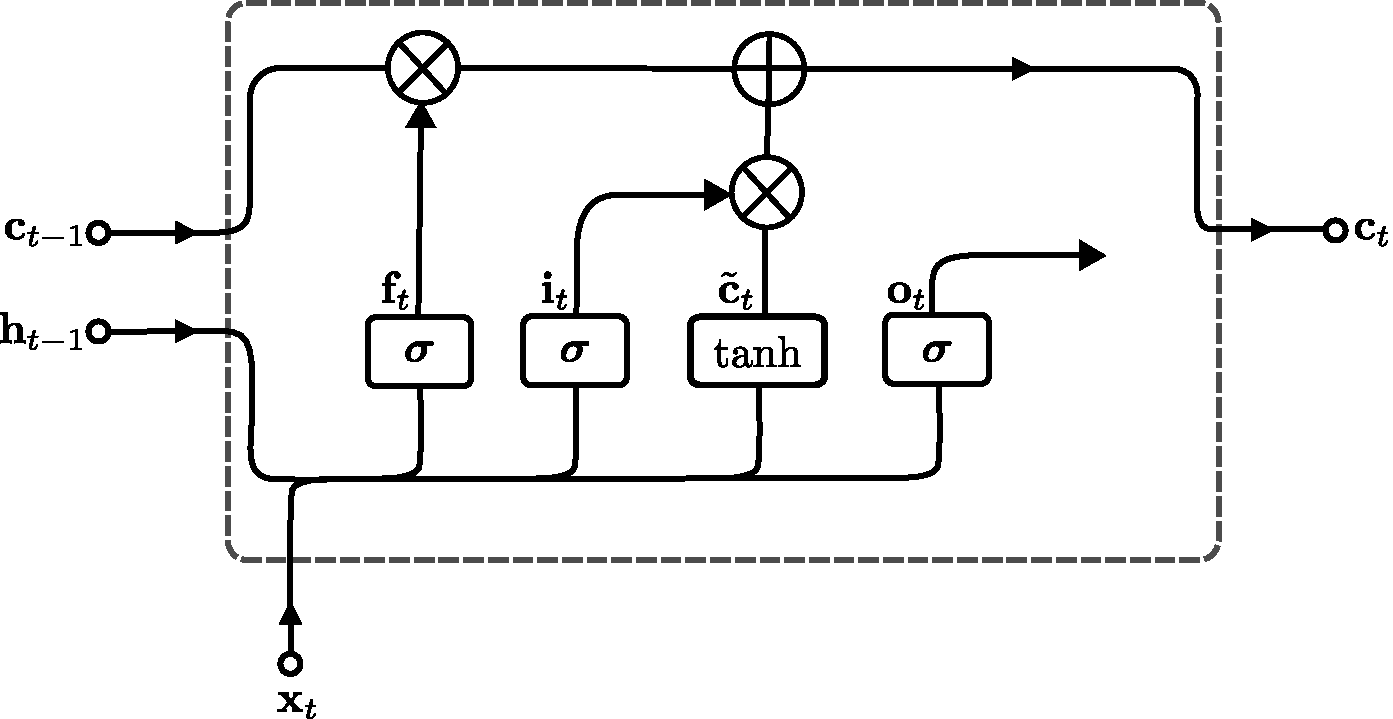
\includegraphics[scale=0.4]{Module 5 (RNN)/pics/LSTM_int_stat2.pdf}
 \end{center} 
 \begin{itemize}
     \item $\bbf_t$ is elementwise  multiplied with internal state $\bc_{t-1}$. 
     \item If the outputs of  $\bbf_t$ are low, a forgetting factor is applied to $\bc_t$. 
     \item At the same time, $\bi_t$ elementwise multiplies  ${\tilde\bc}_t$, and the product is added to  $\bc_{t-1}$ state to produce $\bc_t$.
 \end{itemize}
\end{frame}
\begin{frame}{Structure}{Internal state}
The operation to compute the internal state is 
    \begin{equation}
    \bc_t = \bc_{t-1} \odot \bbf_t + \tilde{\bc}_i \odot \bi_t
\end{equation}
\begin{itemize}
    \item Notice the equivalence of the above structure with  the unit gain self-feedback described as constant error carousel (CEC) in the
original paper by Hochreiter and Schmidhuber. 
\item The backpropagation of the error through the internal state line is done without transformation through any nonlinear function derivative or weight matrix, therefore avoiding the phenomena of vanishing or exploding gradients.
\end{itemize}
\end{frame}
\begin{frame}{Structure}{Hidden state $\bh_t$}
\begin{center}
 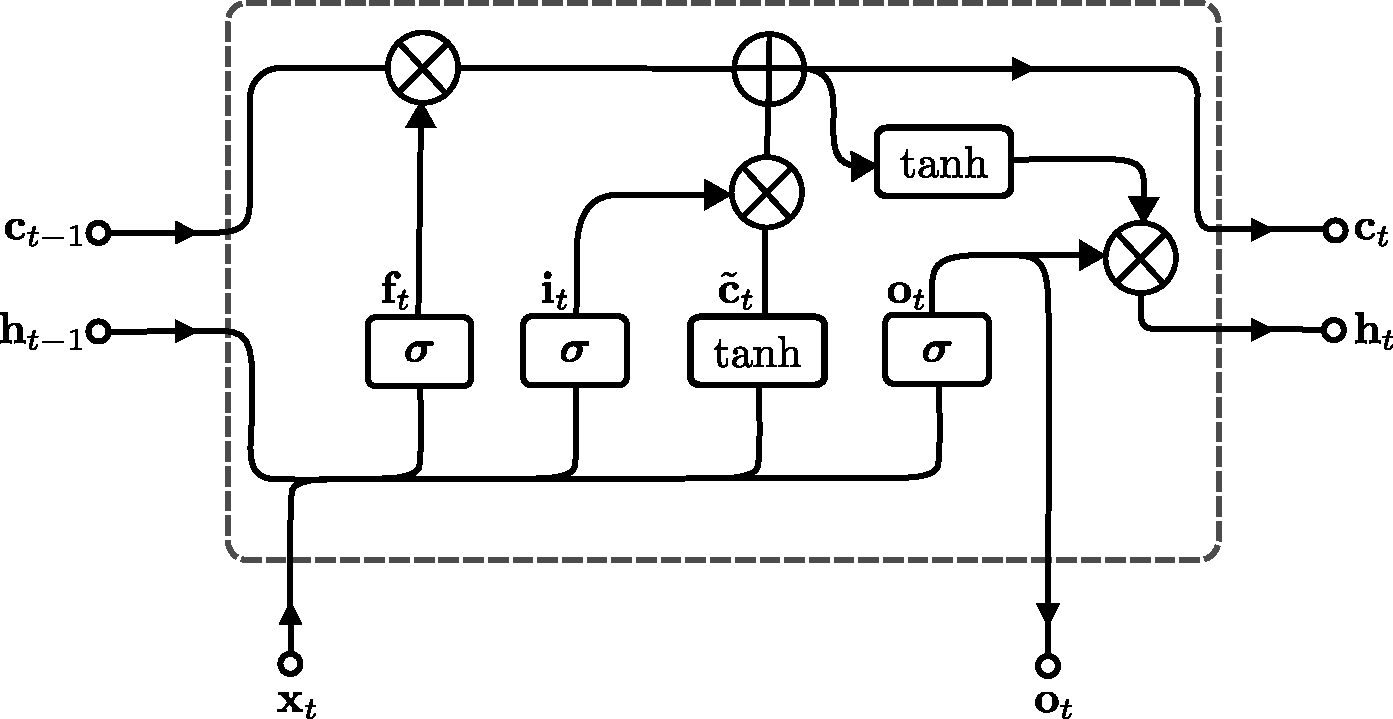
\includegraphics[scale=0.4]{Module 5 (RNN)/pics/Long_Short-Term_Memory.pdf}
 \end{center} 
 \begin{itemize}
 \item The computation of the LSTM ouput gate is
\begin{equation}
\bh_t = \tanh\left(\bc_t \right) \odot \bo_t 
\end{equation}
\end{itemize}
\end{frame}
\begin{frame}{Backpropagation}
\begin{center}
 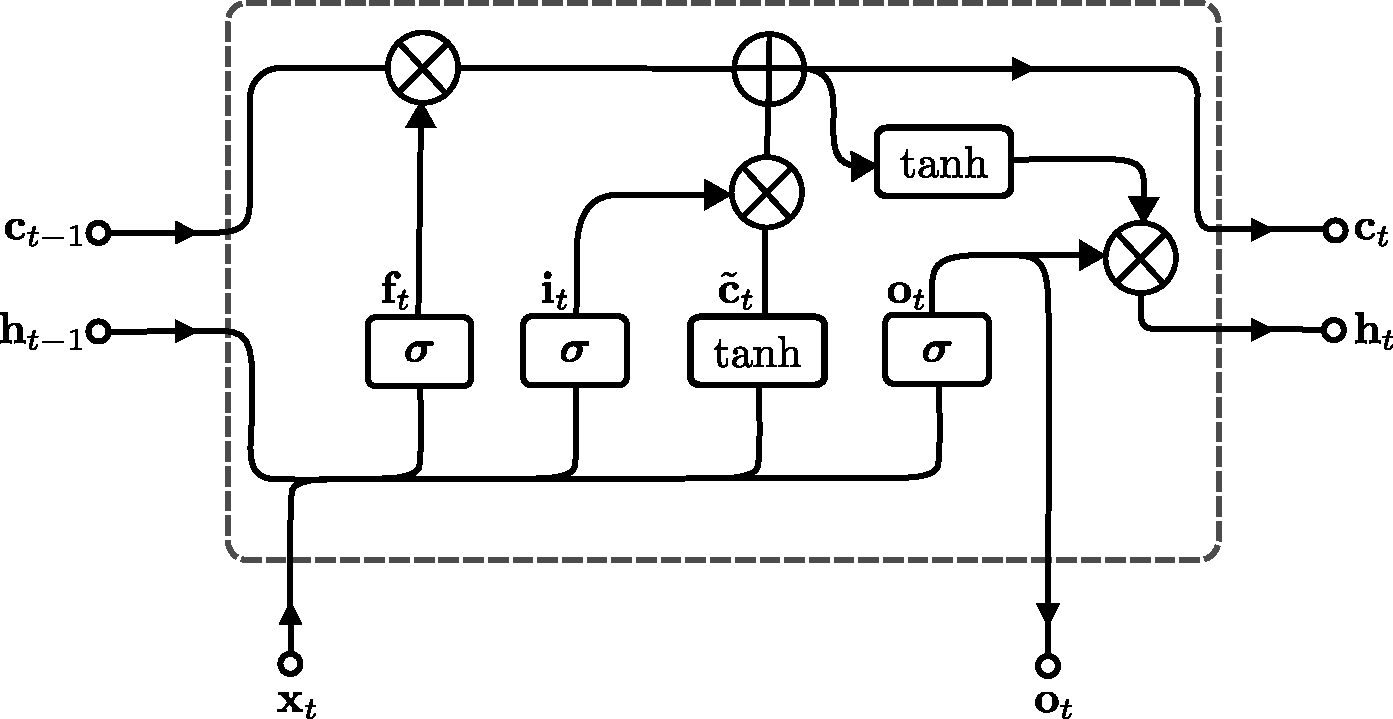
\includegraphics[scale=0.4]{Module 5 (RNN)/pics/Long_Short-Term_Memory.pdf}
 \end{center} 
 \begin{itemize}
     \item The backpropagation through time is computed essentially as in an RNN.
     \item It can be done by following the paths in the direction opposite to the arrows
 \end{itemize}
\end{frame}
\begin{frame}{Backpropagation}

\begin{itemize}
    \item Gradient with respect to the hidden state $\bh_t$
    \begin{equation}
        \nabla_{\bh_t} J_{ML} = \bh_t - \by_t = \bdelta_t
    \end{equation}
    \item Gradient with respect to the output gate $\bo_t$
    \begin{equation}
             \nabla_{\bo_t} J_{ML} =  \bdelta_t \odot \tanh(\bc_t)
    \end{equation}
    \item Gradient with respect to internal state $\bc_t$
    \begin{equation}
         \nabla_{\bc_t} J_{ML} = \bdelta_t \odot {\bo_t} \odot \tanh'(\bc_t)
    \end{equation}
     \begin{equation}
         \nabla_{\bc_{t-1}} J_{ML} = \bdelta_t \odot {\bo_t} \odot \tanh'(\bc_t) \odot{\bbf_t}
    \end{equation}
\end{itemize}
\end{frame}

\begin{frame}{Backpropagation}

\begin{itemize}
    \item Gradient with respect to the input gate $\bi_t$
    \begin{equation}
        \nabla_{\bi_t} J_{ML} = \bdelta_t \odot {\bo_t} \odot \tanh'(\bc_t) \odot {\tilde {\bc}_t}
    \end{equation}
    \item Gradient with respect to the input state $\tilde{\bc}_t$
    \begin{equation}
             \nabla_{\tilde{\bc}_t} J_{ML} =  \bdelta_t \odot {\bo_t} \odot \tanh'(\bc_t) \odot {\bi}_t
    \end{equation}
    \item Gradient with respect to the forgetting gate $\bbf_t$
    \begin{equation}
         \nabla_{\bbf_t} J_{ML} = \bdelta_t \odot {\bo_t} \odot \tanh'(\bc_{t-1})
    \end{equation}
\end{itemize}

All these gradients are used to compute the gradient with respect to the weights. They are 8 matrices and 4 biases. 
\end{frame}
\begin{frame}{Backpropagation}
\begin{itemize}
    \item Gradient with respect to output gate weights:
    \begin{equation}
    \begin{split}        
    \nabla_{\bW_{xo}} J_{ML}  &=  \bdelta_t \odot  \tanh(\bc_t) \odot \bsigma'(\bz_o)\odot \bx_t\\
    \nabla_{\bW_{ho}} J_{ML}  &=  \bdelta_t \odot  \tanh(\bc_t) \odot \bsigma'(\bz_o)\odot \bh_{t-1}\\
   \nabla_{\bb_{o}}  J_{ML} &=  \bdelta_t \odot  \tanh(\bc_t) \odot \bsigma'(\bz_o) \\
    \end{split}
    \end{equation}

\item Gradient with respect to forgetting gate weights:
    \begin{equation}
    \begin{split}        
    \nabla_{\bW_{xf}} J_{ML}  &=  \bdelta_t \odot \bo_t \odot \tanh'(\bc_t) \odot \bc_t \odot \bsigma'(\bz_f)\odot \bx_t\\
    \nabla_{\bW_{hf}}  J_{ML} &=  \bdelta_t \odot  \bo_t \odot \tanh'(\bc_t) \odot \bc_t \odot \bsigma'(\bz_f)\odot \bh_{t-1}\\
   \nabla_{\bb_{f}} J_{ML}  &=  \bdelta_t \odot  \bo_t \odot \tanh'(\bc_t) \odot \bc_t \odot \bsigma'(\bz_f) \\
    \end{split}
    \end{equation}


\end{itemize}
\end{frame}
\begin{frame}{Backpropagation}
\begin{itemize}
    \item Gradient with respect to the input gate weights:
    \begin{equation}
        \begin{split}
        \nabla_{\bW_{xi}} J_{ML} &= \bdelta_t \odot \bo_t \odot \tanh'(\bc_t) \odot \tilde{\bc}_t \odot \bsigma'(\bz_g)  \odot \bx_t\\
    \nabla_{\bW_{hi}} J_{ML} &=  \bdelta_t \odot \bo_t \odot \tanh'(\bc_t) \odot \tilde{\bc}_t \odot \bsigma'(\bz_g)  \odot   \bh_{t-1}\\
    \nabla_{\bb_{bi}} J_{ML} & =  \bdelta_t \odot \bo_t \odot \tanh'(\bc_t) \odot \tilde{\bc}_t \odot \bsigma'(\bz_g) 
        \end{split}
    \end{equation}

    \item Gradient with respect to the input state weights:
 \begin{equation}
    \begin{split}        
    \nabla_{\bW_{xc}} J_{ML}  &=  \bdelta_t \odot \bo_t \odot \tanh'(\bc_t) \odot \bc_t \odot \bsigma'(\bz_f)\odot \bx_t\\
    \nabla_{\bW_{hc}}  J_{ML} &=  \bdelta_t \odot  \bo_t \odot \tanh'(\bc_t) \odot \bc_t \odot \bsigma'(\bz_f)\odot \bh_{t-1}\\
   \nabla_{\bb_{c}} J_{ML}  &=  \bdelta_t \odot  \bo_t \odot \tanh'(\bc_t) \odot \bc_t \odot \bsigma'(\bz_f) \\
    \end{split}
    \end{equation}

\end{itemize}
    
\end{frame}
\end{document}